\iffalse
This file is protected by Copyright. Please refer to the COPYRIGHT file
distributed with this source distribution.

This file is part of OpenCPI <http://www.opencpi.org>

OpenCPI is free software: you can redistribute it and/or modify it under the
terms of the GNU Lesser General Public License as published by the Free Software
Foundation, either version 3 of the License, or (at your option) any later
version.

OpenCPI is distributed in the hope that it will be useful, but WITHOUT ANY
WARRANTY; without even the implied warranty of MERCHANTABILITY or FITNESS FOR A
PARTICULAR PURPOSE. See the GNU Lesser General Public License for more details.

You should have received a copy of the GNU Lesser General Public License along
with this program. If not, see <http://www.gnu.org/licenses/>.
\fi
%----------------------------------------------------------------------------------------
% Update the docTitle and docVersion per document
%----------------------------------------------------------------------------------------
\def\docTitle{FPGA Vendor Tools Installation Guide}
\def\docVersion{1.2}
%----------------------------------------------------------------------------------------
\documentclass{article}
\iffalse
This file is protected by Copyright. Please refer to the COPYRIGHT file
distributed with this source distribution.

This file is part of OpenCPI <http://www.opencpi.org>

OpenCPI is free software: you can redistribute it and/or modify it under the
terms of the GNU Lesser General Public License as published by the Free Software
Foundation, either version 3 of the License, or (at your option) any later
version.

OpenCPI is distributed in the hope that it will be useful, but WITHOUT ANY
WARRANTY; without even the implied warranty of MERCHANTABILITY or FITNESS FOR A
PARTICULAR PURPOSE. See the GNU Lesser General Public License for more details.

You should have received a copy of the GNU Lesser General Public License along
with this program. If not, see <http://www.gnu.org/licenses/>.
\fi
\author{} % Force author to be blank
%----------------------------------------------------------------------------------------
% Paper size, orientation and margins
%----------------------------------------------------------------------------------------
\usepackage{geometry}
\geometry{
        letterpaper, % paper type
        portrait,    % text direction
        left=.75in,  % left margin
        top=.75in,   % top margin
        right=.75in, % right margin
        bottom=.75in % bottom margin
 }
%----------------------------------------------------------------------------------------
% Header/Footer
%----------------------------------------------------------------------------------------
\usepackage{fancyhdr} \pagestyle{fancy} % required for fancy headers
\renewcommand{\headrulewidth}{0.5pt}
\renewcommand{\footrulewidth}{0.5pt}
\rhead{\small{ANGRYVIPER Team}}
% \rfoot{\thepage}
%----------------------------------------------------------------------------------------
% Appendix packages
%----------------------------------------------------------------------------------------
\usepackage[toc,page]{appendix}
%----------------------------------------------------------------------------------------
% Defined Commands & Renamed Commands
%----------------------------------------------------------------------------------------
\renewcommand{\contentsname}{Table of Contents}
\renewcommand{\listfigurename}{List of Figures}
\renewcommand{\listtablename}{List of Tables}
%----------------------------------------------------------------------------------------
% Various packages
%----------------------------------------------------------------------------------------
\usepackage[usenames,dvipsnames]{xcolor} % for color names see https://en.wikibooks.org/wiki/LaTeX/Colors
\usepackage{hyperref}  % for linking urls and lists
\usepackage{graphicx}  % for including pictures by file
\usepackage{listings}  % for coding language styles
\usepackage{rotating}  % for sideways table
\usepackage{pifont}    % for sideways table
\usepackage{pdflscape} % for landscape view
\usepackage{subfig}
\usepackage{xstring}
\uchyph=0 % Never hyphenate acronyms like RCC (I think this overrides ANGRYVIPER above)
\renewcommand\_{\textunderscore\allowbreak} % Allow words to break/newline on underscores
%----------------------------------------------------------------------------------------
% Table packages
%----------------------------------------------------------------------------------------
\usepackage{longtable} % for long possibly multi-page tables
\usepackage{tabularx} % c=center,l=left,r=right,X=fill
% These define tabularx columns "C" and "R" to match "X" but center/right aligned
\newcolumntype{C}{>{\centering\arraybackslash}X}
\newcolumntype{R}{>{\raggedleft\arraybackslash}X}
\usepackage{float}
\floatstyle{plaintop}
\usepackage[tableposition=top]{caption}
\newcolumntype{P}[1]{>{\centering\arraybackslash}p{#1}}
\newcolumntype{M}[1]{>{\centering\arraybackslash}m{#1}}
%----------------------------------------------------------------------------------------
% Block Diagram / FSM Drawings
%----------------------------------------------------------------------------------------
\usepackage{tikz}
\usetikzlibrary{shapes,arrows,fit,positioning}
\usetikzlibrary{automata} % used for the fsm
%----------------------------------------------------------------------------------------
% Colors Used
%----------------------------------------------------------------------------------------
\usepackage{colortbl}
\definecolor{blue}{rgb}{.7,.8,.9}
\definecolor{ceruleanblue}{rgb}{0.16, 0.32, 0.75}
\definecolor{drkgreen}{rgb}{0,0.6,0}
\definecolor{deepmagenta}{rgb}{0.8, 0.0, 0.8}
\definecolor{cyan}{rgb}{0.0,0.6,0.6}
\definecolor{maroon}{rgb}{0.5,0,0}
%----------------------------------------------------------------------------------------
% VHDL Coding Language Style
% modified from: http://latex-community.org/forum/viewtopic.php?f=44&t=22076
%----------------------------------------------------------------------------------------
\lstdefinelanguage{VHDL}
{
        basicstyle=\ttfamily\footnotesize,
        columns=fullflexible,keepspaces,      % https://tex.stackexchange.com/a/46695/87531
        keywordstyle=\color{ceruleanblue},
        commentstyle=\color{drkgreen},
        morekeywords={
    library,use,all,entity,is,port,in,out,end,architecture,of,
    begin,and, signal, when, if, else, process, end,
        },
        morecomment=[l]--
}
%----------------------------------------------------------------------------------------
% XML Coding Language Style
% modified from: http://tex.stackexchange.com/questions/10255/xml-syntax-highlighting
%----------------------------------------------------------------------------------------
\lstdefinelanguage{XML}
{
        basicstyle=\ttfamily\footnotesize,
        columns=fullflexible,keepspaces,
        morestring=[s]{"}{"},
        morecomment=[s]{!--}{--},
        commentstyle=\color{drkgreen},
        moredelim=[s][\color{black}]{>}{<},
        moredelim=[s][\color{cyan}]{\ }{=},
        stringstyle=\color{maroon},
        identifierstyle=\color{ceruleanblue}
}
%----------------------------------------------------------------------------------------
% DIFF Coding Language Style
% modified from http://tex.stackexchange.com/questions/50176/highlighting-a-diff-file
%----------------------------------------------------------------------------------------
\lstdefinelanguage{diff}
{
        basicstyle=\ttfamily\footnotesize,
        columns=fullflexible,keepspaces,
        breaklines=true,                                % wrap text
        morecomment=[f][\color{ceruleanblue}]{@@},      % group identifier
        morecomment=[f][\color{red}]-,                  % deleted lines
        morecomment=[f][\color{drkgreen}]+,             % added lines
        morecomment=[f][\color{deepmagenta}]{---},      % Diff header lines (must appear after +,-)
        morecomment=[f][\color{deepmagenta}]{+++},
}
%----------------------------------------------------------------------------------------
% Python Coding Language Style
% modified from
%----------------------------------------------------------------------------------------
\lstdefinelanguage{python}
{
        basicstyle=\ttfamily\footnotesize,
        columns=fullflexible,keepspaces,
        keywordstyle=\color{ceruleanblue},
        commentstyle=\color{drkgreen},
        stringstyle=\color{orange},
        morekeywords={
    print, if, sys, len, from, import, as, open,close, def, main, for, else, write, read, range,
        },
        comment=[l]{\#}
}
%----------------------------------------------------------------------------------------
% Fontsize Notes in order from smallest to largest
%----------------------------------------------------------------------------------------
%    \tiny
%    \scriptsize
%    \footnotesize
%    \small
%    \normalsize
%    \large
%    \Large
%    \LARGE
%    \huge
%    \Huge

\date{Version \docVersion} % Force date to be blank and override date with version
\title{\docTitle}
\lhead{\docTitle}
%----------------------------------------------------------------------------------------
\usepackage{multirow}
\begin{document}
\maketitle
\thispagestyle{fancy}
\newpage

	\begin{center}
	\textit{\textbf{Revision History}}
		\begin{table}[H]
		\label{table:revisions} % Add "[H]" to force placement of table
			\begin{tabularx}{\textwidth}{|c|X|l|}
			\hline
			\rowcolor{blue}
			\textbf{Revision} & \textbf{Description of Change} & \textbf{Date} \\
		    \hline
		    v1.1 & Initial Release & 3/2017 \\
			\hline
            v1.2 & Updated for ANGRYVIPER Release 1.2 & 8/2017 \\
		    \hline
			\end{tabularx}
		\end{table}
	\end{center}

\newpage

\tableofcontents

\newpage

\section{References}

	This document assumes a basic understanding of the Linux command line (or ``shell") environment. A working knowledge of ANGRYVIPER is required for understanding what vendor tools are necessary to perform various ANGRYVIPER operations. However, no ANGRYVIPER knowledge is required to perform the toolset installation and configuration herein. The reference(s) in Table \ref{table:references} can be used as an overview of ANGRYVIPER and may prove useful.
\def\refcapbottom{}
\iffalse
This file is protected by Copyright. Please refer to the COPYRIGHT file
distributed with this source distribution.

This file is part of OpenCPI <http://www.opencpi.org>

OpenCPI is free software: you can redistribute it and/or modify it under the
terms of the GNU Lesser General Public License as published by the Free Software
Foundation, either version 3 of the License, or (at your option) any later
version.

OpenCPI is distributed in the hope that it will be useful, but WITHOUT ANY
WARRANTY; without even the implied warranty of MERCHANTABILITY or FITNESS FOR A
PARTICULAR PURPOSE. See the GNU Lesser General Public License for more details.

You should have received a copy of the GNU Lesser General Public License along
with this program. If not, see <http://www.gnu.org/licenses/>.
\fi

% This snippet creates the "References" table labeled "table:references"
% It creates three columns: Name, Publisher, Link and then inserts default documents
%
% To skip these defaults, define macros named
% refskipgs to skip "Getting Started"
% refskipig to skip "Installation Guide"
% refskipac to skip "Acronyms and Definitions"
% refskipocpiov to skip "OpenCPI Overview"
%
% See RPM_Installation_Guide.tex for examples
%
% After the defaults, it optionally inserts the "myreferences" macro that
% you defined elsewhere (you put hlines above all lines)
%
% If you want the \caption on the bottom, define "refcapbottom"
\begin{center}
\renewcommand*\footnoterule{} % Remove separator line from footnote
\renewcommand{\thempfootnote}{\arabic{mpfootnote}} % Use Arabic numbers (or can't reuse)
\begin{minipage}{0.9\textwidth}
  \begin{table}[H]
\ifx\refcapbottom\undefined
  \caption {References}
  \label{table:references}
\fi
  \begin{tabularx}{\textwidth}{|C|C|}
    \hline
    \rowcolor{blue}
    \textbf{Title} & \textbf{Link} \\
\ifx\refskipocpiov\undefined
    \hline
    OpenCPI Overview & \githubio{Overview.pdf} \\
\fi
\ifx\refskipac\undefined
    \hline
    Acronyms and Definitions & \githubio{Acronyms\_and\_Definitions.pdf} \\
\fi
\ifx\refskipgs\undefined
    \hline
    Getting Started & \githubio{Getting\_Started.pdf} \\
\fi
\ifx\refskipig\undefined
    \hline
    Installation Guide & \githubio{RPM\_Installation\_Guide.pdf} \\
\fi
\ifx\myreferences\undefined
\else
    \myreferences
\fi
    \hline
  \end{tabularx}
\ifx\refcapbottom\undefined
\else
  \caption {References}
  \label{table:references}
\fi
  \end{table}
\end{minipage}
\end{center}


\begin{flushleft}
\begin{landscape}
\section{ANGRYVIPER Vendor Tool Prerequisites}
\label{sec:doc_overview}
One or more third party vendor toolsets are required to perform various ANGRYVIPER operations. Table~\ref{table:tool-support} identifies the various possible vendor tool installation and license requirement combinations. Each combination enumerates the associated functionality that the given combination provides to ANGRYVIPER. ANGRYVIPER supports Xilinx Vivado 2017.1 with Xilinx Vivado (SDK Only) 2013.4 (explained in \ref{sec:viv_intro}). Testing has been done with Vivado 2015.4, but future regression testing will be performed against 2017.1. ANGRYVIPER also supports Xilinx ISE 14.7, Xilinx LabTools 14.7, and Altera Quartus 15.1.
%Commented this out because there may be other Vivado functionality that requires a non-webpack license.
%Maximum functionality for ANGRYVIPER's currently supported platforms is provided by a WebPACK licensed Xilinx Vivado installation, a non-WebPACK licensed Xilinx ISE installation and a licensed Quartus installation.

\begin{center}
	\renewcommand*\footnoterule{} % Remove separator line from footnote
	\renewcommand{\thempfootnote}{\arabic{mpfootnote}} % Use Arabic numbers (or can't reuse)
	\begin{table}[H]
		\caption {Support with Vendor Tools}
		\label{table:tool-support} % Add "[H]" to force placement of table
		\newcolumntype{Z}{>{\raggedright\arraybackslash}X}
		\def\arraystretch{1.5}
		\begin{tabularx}{1.35\textwidth}{| c | Z | p{1.8cm} | p{2.9cm} | p{3.6cm} | p{3cm} | Z |}
			\hline
			\rowcolor{blue}
			\textbf{Tool} & \multicolumn{1}{|c|}{\textbf{Installation}} & \textbf{Supported \newline simulators} & \textbf{Load bitstreams onto} & \textbf{Run applications on these platforms} & \textbf{Build bitstreams for} & \textbf{Build software for} \\
			\hline
			\multicolumn{2}{|c|}{\textbf{No vendor tools}} & & Zynq$^1$ & Zynq-based$^2$, x86-only$^1$ & & x86$^1$ \\
			\hline
			\multirow{3}{*}[-2em]{\textbf{Xilinx Vivado}} & 2017.1 with WebPACK License & \code{xsim} & & & Zynq$^3$ & \\ \cline{2-7}
			& 2013.4 (SDK only) & & & & & Zynq-ARM \\ \cline{2-7}
			& 2017.1 \textit{and} 2013.4 SDK with WebPACK License & \code{xsim} & & & Zynq$^3$ &  Zynq-ARM \\
			\hline
			\multicolumn{2}{|c|}{\textbf{Xilinx LabTools 14.7}} & & ML605 & x86/ML605 & & \\
			\hline
			\multirow{2}{*}{\textbf{Xilinx ISE 14.7}} & WebPACK License & \code{isim} & ML605 & x86/ML605 & Zynq$^3$ & Zynq-ARM \\ \cline{2-7}
			& Full License & \code{isim} & ML605 & x86/ML605 & Zynq, ML605 & Zynq-ARM \\
			\hline
			\multicolumn{2}{|c|}{\textbf{Altera Quartus 15.1 with License}}  & \code{modelsim} & ALST4 & x86/ALST4 & ALST4 & \\
			\hline
		\end{tabularx}\newline

		\footnotesize{$^1$With ANGRYVIPER installed, no additional software is required to load bitstreams onto Zynq FPGAs, run applications on Zynq-based or x86-only platforms, or build software for x86.}\\
		\footnotesize{$^2$``Zynq-based'' platform includes both a Zynq's FPGA and ARM PS. The usage of ``Zynq'' or ``Zynq-based'' here does not include Zynq UltraScale devices.}\\
		\footnotesize{$^3$Building bitstreams with a WebPACK license is limited to certain Zynq parts. Refer to the vendor's documentation for further information.}\\
	\end{table}
\end{center}
\end{landscape}

\section{Xilinx Toolset Installation and Configuration}
\subsection{Xilinx Vivado Installation in CentOS~6/7}
\label{sec:viv_intro}
\begin{flushleft}
In order to use Vivado with ANGRYVIPER, it is required that you install Vivado 2017.1 \textit{and} Vivado 2013.4's SDK. The 2013.4 SDK is necessary because ANGRYVIPER's ``\code{xilinx13\_3}'' software platform requires an SDK with matching glibc/glibc++ versions. An SDK meeting this requirement can be found explicitly in either ISE 14.7 or Vivado 2013.4 SDK. For more information on this requirement you can reference the README for the \code{xilinx13\_3} software platform. This is located in the CDK (\textit{e.g.}: \path{/opt/opencpi/cdk/platforms/xilinx13_3}).
\subsubsection{Xilinx Vivado 2017.1 Installation in CentOS~6/7}
\label{sec:viv}
\begin{enumerate}
\item Download the Vivado 2017.1 installation files from Xilinx's download site:
\url{https://www.xilinx.com/support/download/index.html/content/xilinx/en/downloadNav/vivado-design-tools/2017-1.html}. A Xilinx account will be required.
\begin{figure}[ht]
	\centerline{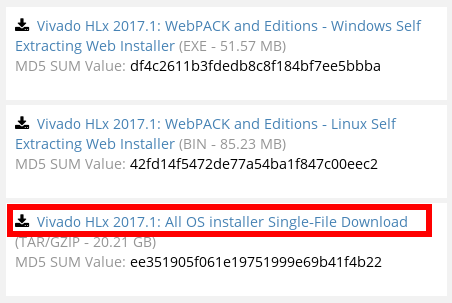
\includegraphics[scale=0.6]{figures/xilinx_vivado_2017_download}}
	\caption{Xilinx Vivado 2017.1 Download}
\end{figure}
\item Extract the tarball:\newline
\code{\% tar -xf Xilinx\_Vivado\_SDK\_2017.1\_0415\_1.tar.gz}
\item Enter the resulting directory and run the installer:\newline
\code{\% cd Xilinx\_Vivado\_SDK\_2017.1\_0415\_1}\newline
\code{\% ./xsetup}\newline
Execution of this file will likely require root privileges (i.e. \code{sudo}).
\pagebreak
\item Run through the installation process. Refer to the images below when applicable.
\begin{figure}[H]
	\centerline{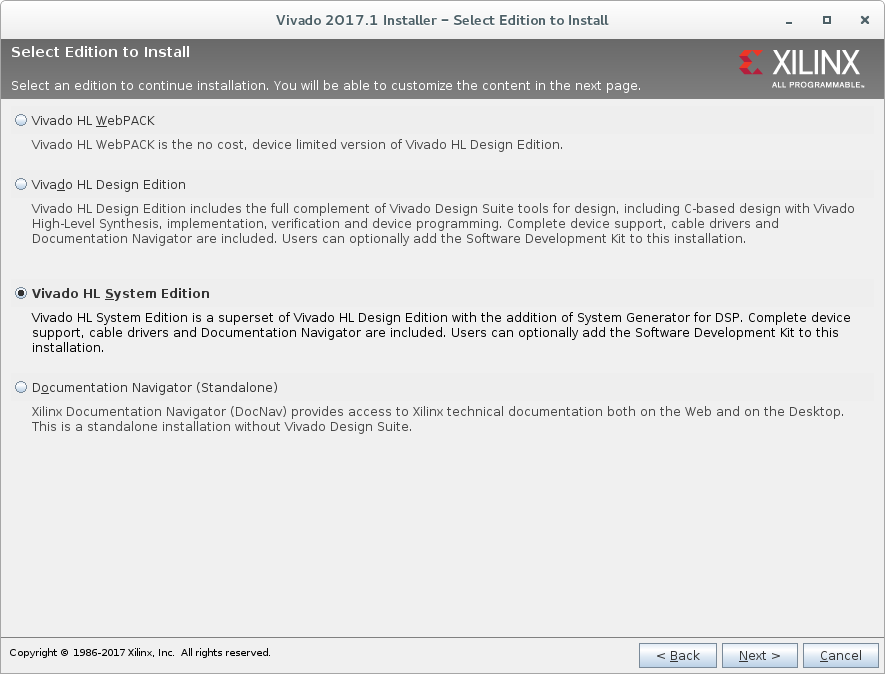
\includegraphics[scale=0.4]{figures/xilinx_vivado_2017_install}}
	\caption{Xilinx Vivado Installer}
\end{figure}
We do not direct you to acquire a license, but if you do not already have one, you will need to select ``Acquire or Manage a License Key'' in the image below.
\begin{figure}[H]
	\centerline{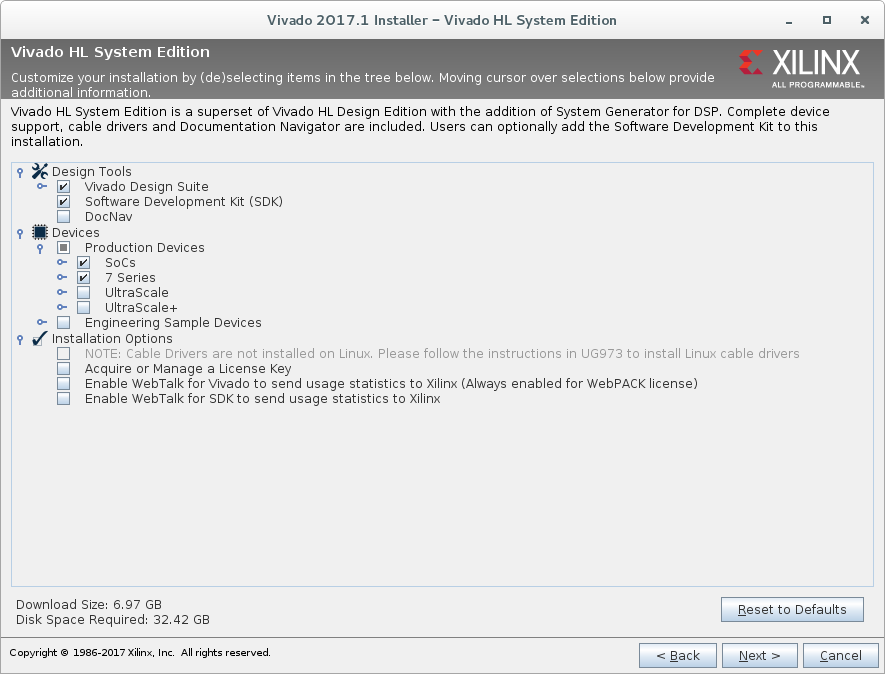
\includegraphics[scale=0.4]{figures/xilinx_vivado_2017_choose_installation}}
	\caption{Xilinx Vivado Installation Choice}
\end{figure}
\pagebreak
Take note of the installation directory chosen (e.g. \code{/opt/Xilinx}) as well as the Vivado version (e.g. \code{2017.1}) for later use.
\begin{figure}[H]
	\centerline{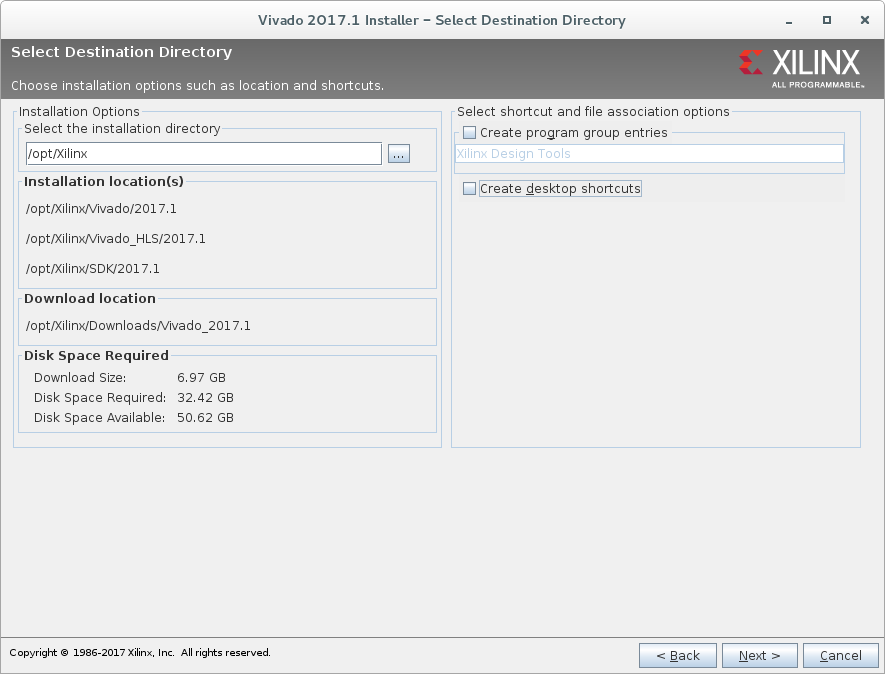
\includegraphics[scale=0.4]{figures/xilinx_vivado_2017_install_location}}
	\caption{Xilinx Vivado Install Location}
\end{figure}
\end{enumerate}
\subsubsection{ANGRYVIPER Considerations}
\begin{enumerate}
\item Note that sourcing the ``\verb+<Vivado-install-dir>/Vivado/<Vivado-version>/settings64.sh+'' script will interfere with ANGRYVIPER's environment setup. Accordingly, it is recommended to always source these scripts and execute any follow-on commands in a \textit{separate terminal}.
\item To use ANGRYVIPER with any Xilinx Vivado installation, it is required to set the following environment variables before running ANGRYVIPER commands. Note that each of the following \code{export} statements is only necessary under the following conditions:
\begin{itemize}
\item When using a non-default installation location (i.e. anything other than \path{/opt/Xilinx})
\item When Vivado \textit{and} ISE are both being used and are installed in different locations
\item Or when multiple versions of Vivado are installed and you wish to use a version other than the newest.
\end{itemize}

\subitem \code{\% export OCPI\_XILINX\_VIVADO\_DIR=<Vivado-install-dir>}
\subitem \code{\% export OCPI\_XILINX\_VIVADO\_VERSION=<Vivado-version>}

\end{enumerate}
If ANGRYVIPER has been installed prior to the Vivado installation, and it is desired to make the aforementioned environment variables set automatically upon login for all users, the variables should be added in \code{/opt/opencpi/cdk/env.d/xilinx.sh}. Logging out and logging back into the user account will apply said variables.
\subsubsection{Xilinx Vivado 2013.4 SDK Only Installation in CentOS~6/7}
\label{sec:viv_sdk}
\begin{enumerate}
\item Download the Vivado 2013.4 Standalone SDK installation files from Xilinx's download site:
\url{https://www.xilinx.com/support/download/index.html/content/xilinx/en/downloadNav/vivado-design-tools/archive.html}. Navigate to ``2013.4'' $\rightarrow$ ``Software Development Kit''. A Xilinx account will be required.

\begin{figure}[H]
	\centerline{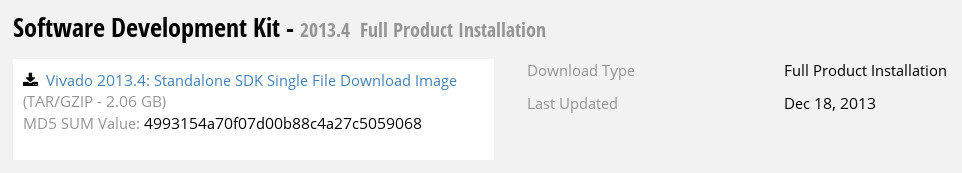
\includegraphics[scale=0.4]{figures/xilinx_vivado_sdk_download}}
	\caption{Xilinx Vivado 2013.4 SDK Download}
\end{figure}
\item Extract the tarball:\newline
\code{\% tar -xf Xilinx\_SDK\_2013.4\_1210\_1.tar}
\item Enter the resulting directory and run the installer:\newline
\code{\% cd Xilinx\_SDK\_2013.4\_1210\_1}\newline
\code{\% ./xsetup}\newline
Execution of this file will likely require root privileges (i.e. \code{sudo}).
\pagebreak
\item Run through the installation process. Refer to the images below when applicable.
\begin{figure}[H]
	\centerline{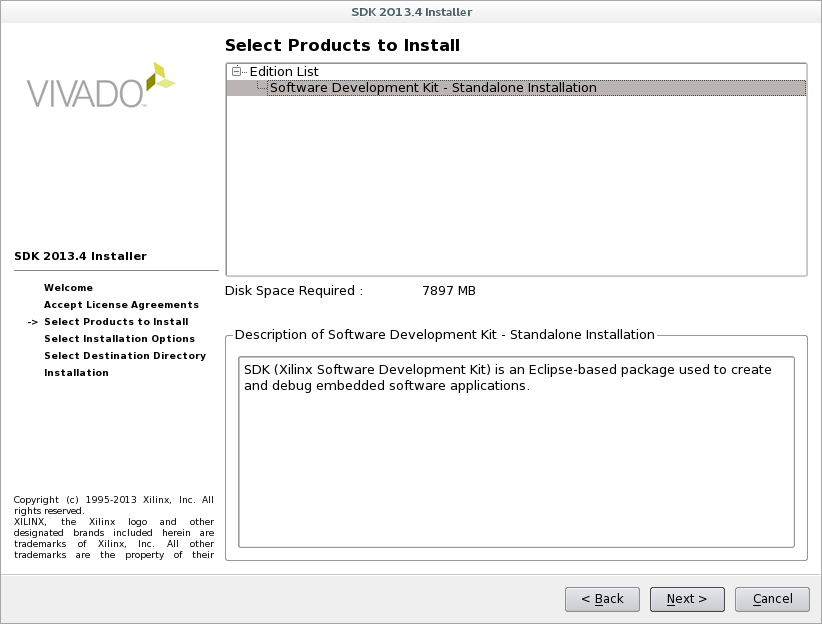
\includegraphics[scale=0.4]{figures/xilinx_vivado_sdk_install}}
	\caption{Xilinx Vivado SDK Installer}
\end{figure}

\begin{figure}[H]
	\centerline{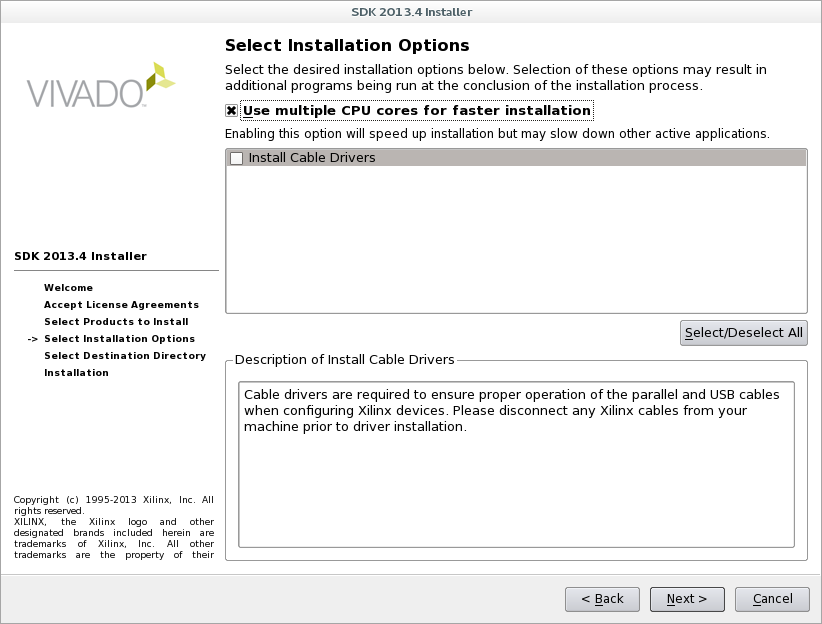
\includegraphics[scale=0.4]{figures/xilinx_vivado_sdk_choose_installation}}
	\caption{Xilinx Vivado SDK Installation Choice}
\end{figure}
\pagebreak
Take note of the installation directory chosen (e.g. \code{/opt/Xilinx}) as well as the Vivado version (e.g. \code{2013.4}) for later use.
\begin{figure}[H]
	\centerline{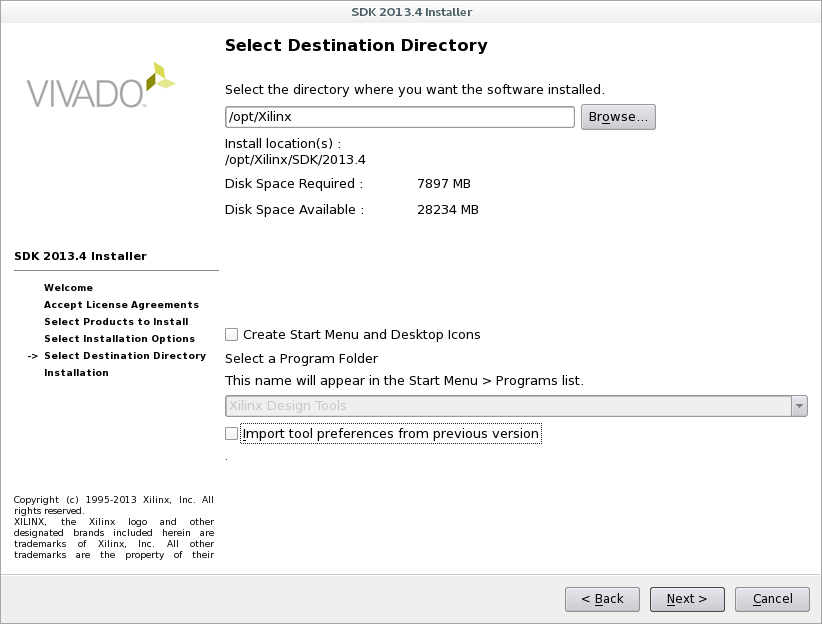
\includegraphics[scale=0.4]{figures/xilinx_vivado_sdk_install_location}}
	\caption{Xilinx Vivado SDK Install Location}
\end{figure}
\end{enumerate}
\end{flushleft}

\subsection{Xilinx ISE 14.7 Installation in CentOS~6/7}
\label{sec:ise}
\begin{flushleft}
\begin{enumerate}
\item Download the ISE 14.7 installation files from Xilinx's download site:
\url{https://www.xilinx.com/support/download/index.html/content/xilinx/en/downloadNav/design-tools.html}. A Xilinx account will be required.
\begin{figure}[ht]
	\centerline{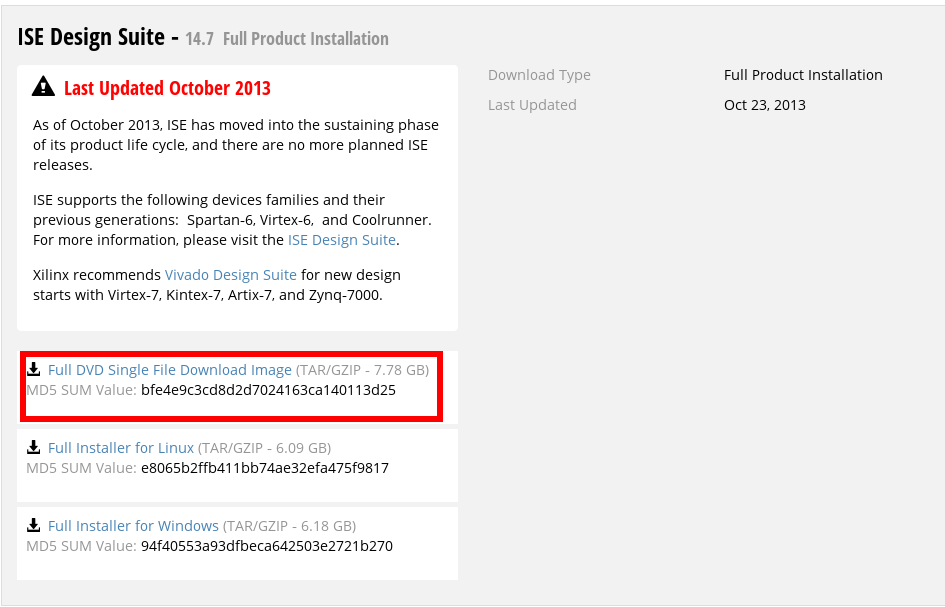
\includegraphics[scale=0.4]{figures/xilinx_ise_download}}
	\caption{Xilinx ISE Download}
\end{figure}
\item Extract the tarball:\newline
\code{\% tar -xf Xilinx\_ISE\_DS\_14.7\_1015\_1.tar}
\item Enter the resulting directory and run the installer:\newline
\code{\% cd Xilinx\_ISE\_DS\_14.7\_1015\_1}\newline
\code{\% ./xsetup}\newline
Execution of this file will likely require root privileges (i.e. \code{sudo}).
\pagebreak
\item Run through the installation process. Refer to the images below when applicable. Note that the checkbox for cable drivers is left unchecked. Cable driver installation, if necessary, should be handled after this installation is complete. See section \ref{sec:cable} for more information.
\begin{figure}[H]
	\centerline{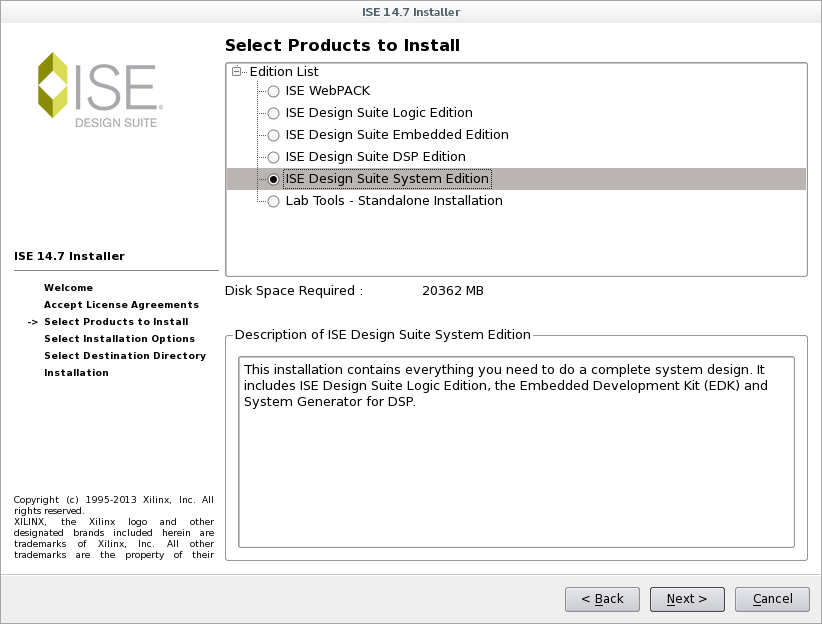
\includegraphics[scale=0.4]{figures/xilinx_ise_install}}
	\caption{Xilinx ISE Installer}
\end{figure}

\begin{figure}[H]
	\centerline{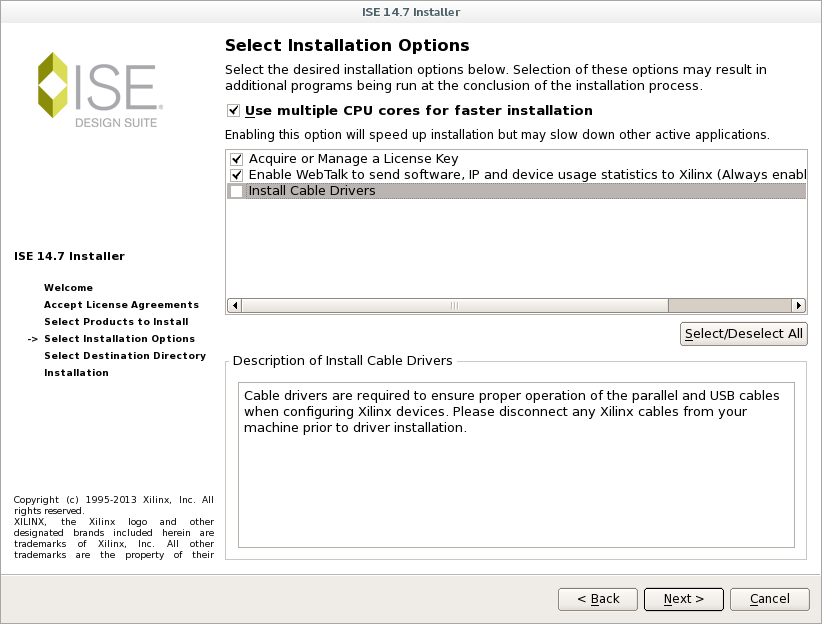
\includegraphics[scale=0.4]{figures/xilinx_labtools_choose_installation}}
	\caption{Xilinx ISE Installation Choice}
\end{figure}
\pagebreak
Take note of the installation directory chosen (e.g. \code{/opt/Xilinx}) as well as the LabTools version (e.g. \code{14.7}) for later use.
\begin{figure}[H]
	\centerline{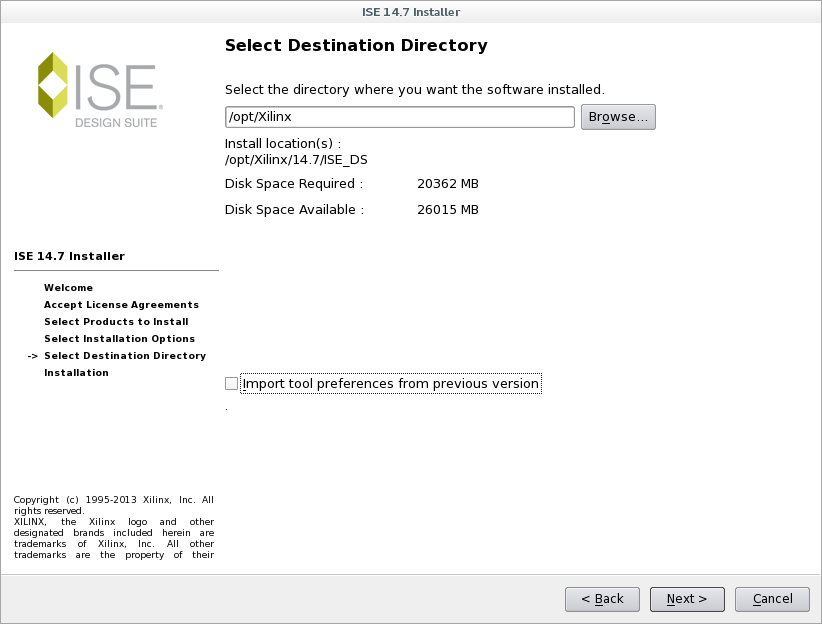
\includegraphics[scale=0.4]{figures/xilinx_ise_install_location}}
	\caption{Xilinx ISE Install Location}
\end{figure}
\end{enumerate}


\subsubsection{ANGRYVIPER Considerations}
\label{sec:iseav}
\begin{enumerate}
\item Note that sourcing the ``\verb+<ISE-install-dir>/<version>/LabTools/settings64.sh+'' or ``\verb+<ISE-install-dir>/<version>/LabTools/settings32.sh+'' scripts will interfere with ANGRYVIPER's environment setup. Accordingly, it is recommended to always source these scripts and execute any follow-on commands in a \textit{separate terminal}.
\item To use ANGRYVIPER with any Xilinx ISE or LabTools installation,  it is required to set the following environment variables before running ANGRYVIPER commands. Note that each of the following \code{export} statements are only necessary when the non-default installation location (i.e. anything other than \path{/opt/Xilinx}) or non-default version (i.e. anything other than \path{14.7}) of the tools were used.
\subitem If only one of Xilinx ISE or Xilinx LabTools is installed,
\subsubitem \code{\% export OCPI\_XILINX\_DIR=<ISE-or-LabTools-install-dir>}
\subsubitem \code{\% export OCPI\_XILINX\_VERSION=<ISE-or-LabTools-version>}
\subitem If Xilinx LabTools and ISE are the same version and installed in the same directory,
\subsubitem \code{\% export OCPI\_XILINX\_DIR=<ISE-and-LabTools-install-dir>}
\subsubitem \code{\% export OCPI\_XILINX\_VERSION=<ISE-and-LabTools-version>}
\subitem If Xilinx LabTools and ISE are the same version and are installed in different directories,
\subsubitem \code{\% export OCPI\_XILINX\_DIR=<ISE-install-dir>}
\subsubitem \code{\% export OCPI\_XILINX\_LAB\_TOOLS\_DIR=<LabTools-install-dir>}
\subsubitem \code{\% export OCPI\_XILINX\_VERSION=<ISE-and-LabTools-version>}
\subitem If Xilinx LabTools and ISE are different versions (LabTools will be ignored),
\subsubitem \code{\% export OCPI\_XILINX\_DIR=<ISE-install-dir>}
\subsubitem \code{\% export OCPI\_XILINX\_VERSION=<ISE-version>}
\end{enumerate}

If ANGRYVIPER has been installed prior to the ISE installation, and it is desired to make the aforementioned environment variables set automatically upon login for all users, the variables should be added in \code{/opt/opencpi/cdk/env.d/xilinx.sh}. Logging out and logging back into the user account will apply said variables.
\end{flushleft}

\subsection{Xilinx LabTools 14.7 Installation in CentOS~6/7}
\label{sec:labtools}
\begin{flushleft}
\begin{enumerate}
\item Download the LabTools 14.7 installation files from Xilinx's download site:
\url{https://www.xilinx.com/support/download/index.html/content/xilinx/en/downloadNav/design-tools.html}. A Xilinx account will be required.
\begin{figure}[H]
	\centerline{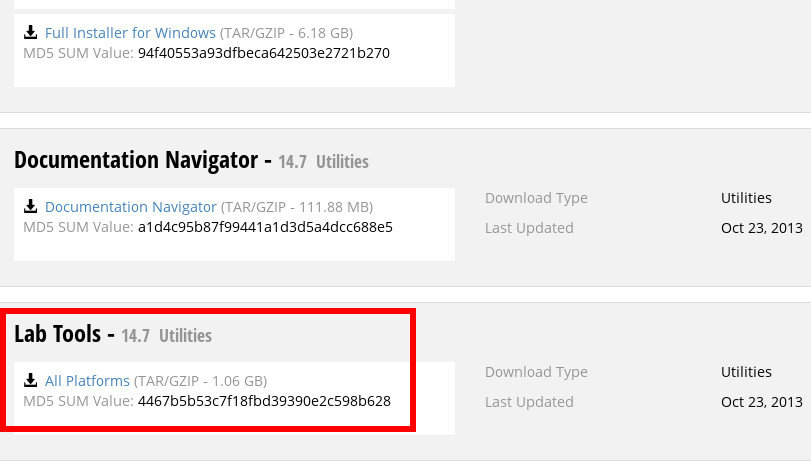
\includegraphics[scale=0.4]{figures/xilinx_labtools_download}}
	\caption{Xilinx LabTools Download}
\end{figure}
\item Extract the tarball:\newline
\code{\% tar -xf Xilinx\_LabTools\_14.7\_1015\_1.tar}
\item Enter the resulting directory and run the installer:\newline
\code{\% cd Xilinx\_LabTools\_14.7\_1015\_1}\newline
\code{\% ./xsetup}\newline
Execution of this file will likely require root privileges (i.e. \code{sudo}).
\pagebreak
\item Run through the installation process. Refer to the images below when applicable. Note that the checkbox for cable drivers is left unchecked. Cable driver installation, if necessary, should be handled after this installation is complete. See section \ref{sec:cable} for more information.
\begin{figure}[H]
	\centerline{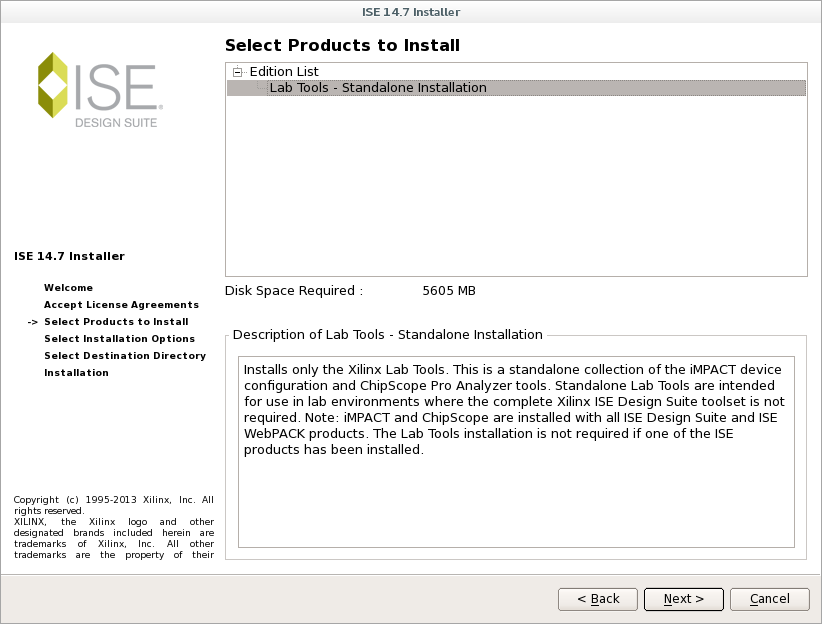
\includegraphics[scale=0.4]{figures/xilinx_labtools_install}}
	\caption{Xilinx LabTools Installer}
\end{figure}
\begin{figure}[H]
	\centerline{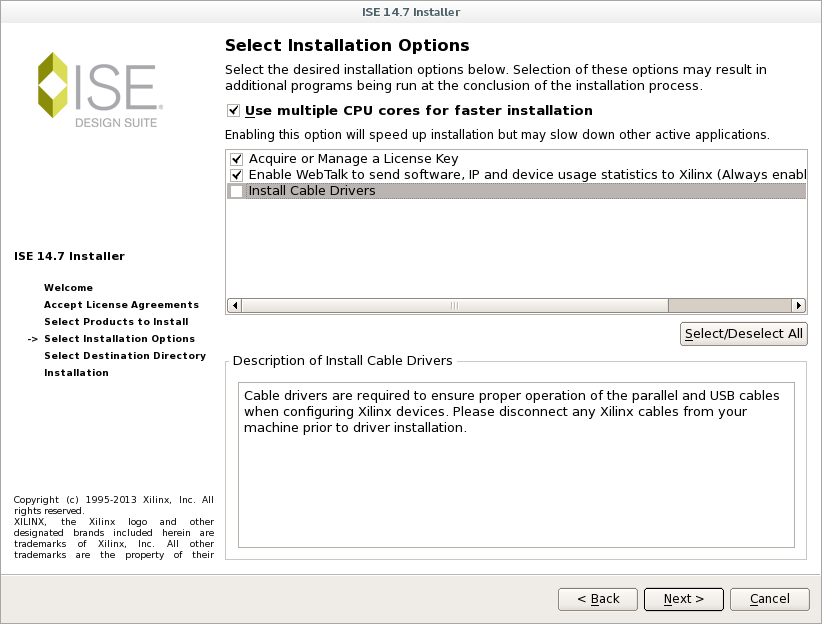
\includegraphics[scale=0.4]{figures/xilinx_labtools_choose_installation}}
	\caption{Xilinx LabTools Installation Choice}
\end{figure}
\pagebreak
Take note of the installation directory chosen (e.g. \code{/opt/Xilinx}) as well as the LabTools version (e.g. \code{14.7}) for later use.
\begin{figure}[H]
	\centerline{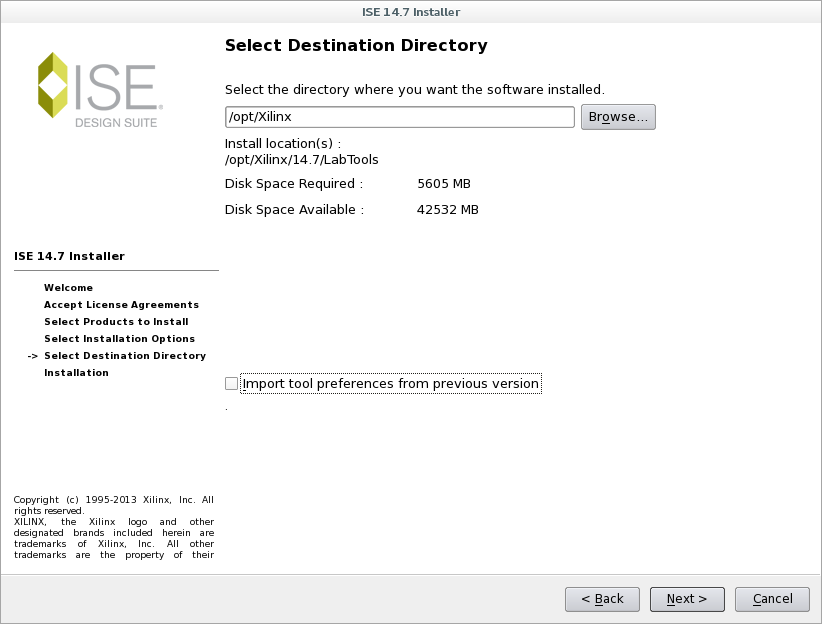
\includegraphics[scale=0.4]{figures/xilinx_labtools_install_location}}
	\caption{Xilinx LabTools Install Location}
\end{figure}
\end{enumerate}

\subsubsection{ANGRYVIPER Considerations}
\begin{enumerate}
\item Note that sourcing the ``\verb+<LabTools-install-dir>/<version>/LabTools/settings64.sh+'' or ``\verb+<LabTools-install-dir>/<version>/LabTools/settings32.sh+'' scripts will interfere with ANGRYVIPER's environment setup. Accordingly, it is recommended to always source these scripts and execute any follow-on commands in a \textit{separate terminal}.
\item To use ANGRYVIPER with any Xilinx ISE or LabTools installation, it is required to set the environment variables according to Section \ref{sec:iseav} before running ANGRYVIPER commands.
\end{enumerate}

\end{flushleft}
\pagebreak

\end{flushleft}

\subsection{Xilinx Toolset Licensing}
\label{xilinx}
A license, either WebPACK or non-WebPACK, is required for Xilinx Vivado and Xilinx ISE. Xilinx LabTools does not require a license.
\begin{enumerate}
\item The following screenshots show an ISE WebPACK license. Refer to \ref{sec:doc_overview} to determine which license is necessary. To generate a license, navigate to \url{http://www.xilinx.com/getlicense} and login (or create an account). Generate a license file:

\begin{figure}[H]
	\centerline{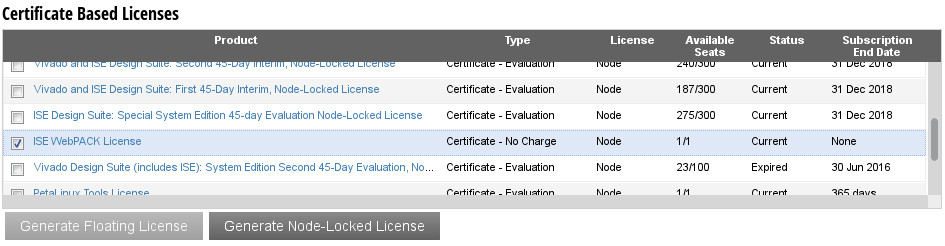
\includegraphics[scale=0.5]{./figures/xilinx_license_gen.jpg}}
	\caption{Generate Xilinx license file}
\end{figure}

\item Download the file and move it to the intended location:

\begin{figure}[H]
	\centerline{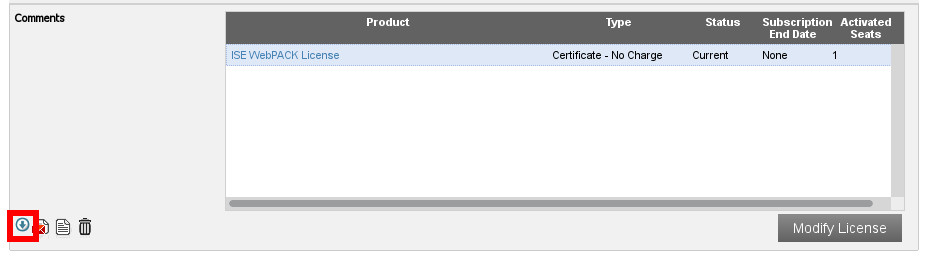
\includegraphics[scale=0.5]{./figures/xilinx_license_download.jpg}}
	\caption{Download Xilinx license file}
\end{figure}
\end{enumerate}

For use of Xilinx tools separate from ANGRYVIPER, you will need to enable the license through the Xilinx tools.\newline

For Vivado, follow these steps:
\begin{enumerate}

\item Run ``\verb+source <Vivado-install-dir>/Vivado/<version>/settings64.sh+''.

\item Open up the license manager and load the downloaded license. The license manager can be launched either from the Vivado GUI, or from the command line by running: \\\verb+sudo <Vivado-install-dir>/Vivado/<version>/bin/vlm+\newline

Here, you can either navigate to ``Load License'' and load a copy of the license file, or you can enter the license search paths via ``Manage License Search Paths''.

\begin{figure}[H]
	\centerline{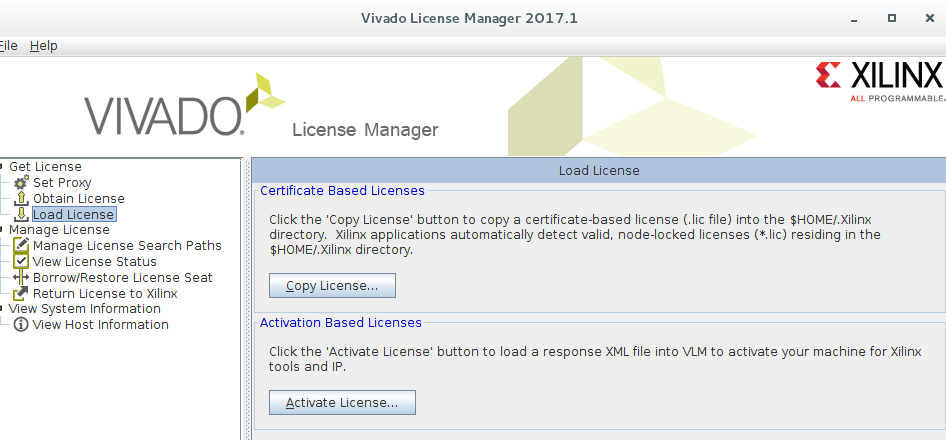
\includegraphics[scale=0.5]{./figures/xilinx_vivado_license_load}}
	\caption{Load Xilinx Vivado license file}
\end{figure}
\end{enumerate}

For ISE, follow these steps:
\begin{enumerate}
\item Run ``\verb+source <ISE-install-dir>/<version>/ISE_DS/settings64.sh+'' (or settings32.sh if the system has a 32-bit architecture).

\item Open up the license manager and load the downloaded license. The license manager can either be launched from the ISE GUI, or launched from the command line by running: \\\verb+sudo <ISE-or-LabTools-install-dir>/<version>/ISE_DS/common/bin/lin[64]/xlcm+

\begin{figure}[H]
	\centerline{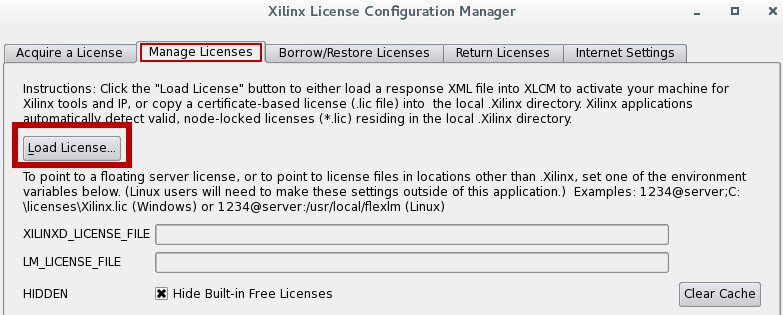
\includegraphics[scale=0.5]{./figures/xilinx_license_load.jpg}}
	\caption{Load Xilinx ISE license file}
\end{figure}
\end{enumerate}

\subsubsection{Note on node-locked licenses in CentOS~7}
If using a Xilinx node-locked license under CentOS~7, see \href{https://access.redhat.com/documentation/en-US/Red_Hat_Enterprise_Linux/7/html/Networking_Guide/sec-Disabling_Consistent_Network_Device_Naming.html}{the Red Hat Networking Guide} to revert to the
\texttt{eth\textit{N}} naming convention.

\subsubsection{ANGRYVIPER Considerations}
\begin{enumerate}
\item Note that sourcing the ``\verb+settings64.sh+'' or ``\verb+settings32.sh+'' scripts will interfere with ANGRYVIPER's environment setup. Accordingly, it is recommended to always source these scripts and execute any follow-on commands in a \textit{separate terminal}.
\item To enable a license for use through ANGRYVIPER, the following is required:

	\begin{itemize}
		\item Add \verb+export OCPI_XILINX_LICENSE_FILE=<PATH_TO_LIC>+ to \verb+/opt/opencpi/cdk/env.d/xilinx.sh+. Note that this can instead point to a license server \verb+<port>@<server.ip.addr>+. If using a floating license server, it is possible to set \verb+OCPI_XILINX_LICENSE_FILE+ to the license server in addition to setting \\\verb+export XILINXD_LICENSE_FILE=<PATH_TO_LOCAL_LIC>+. This will allow use of a local license, e.g. a local WebPACK license, by default and the served floating license when WebPACK license is not sufficient.\footnote{See Xilinx ``\href{https://www.xilinx.com/support/answers/42507.html}{AR\# 42507: What are the search order and locations...}'' and ``\href{https://www.xilinx.com/support/answers/44024.html}{AR\# 44024: If a feature is licensed in multiple locations...}''}
	\end{itemize}
\end{enumerate}

\subsection{Xilinx Cable Driver Installation in CentOS~6/7}
\label{sec:cable}
\subsubsection{Vivado}
\begin{flushleft}
The steps herein are a slightly modified subset of those outlined in \url{https://www.xilinx.com/support/answers/66440.html}.
\end{flushleft}
\begin{enumerate}
\item Run the following command : \code{ls -al /etc/udev/rules.d}
\item Check if the following two files are present : \code{52-digilent-usb.rules 52-xilinx-pcusb.rules}
\item If the files above are not present, run the installer (\textit{it is important to have the JTAG cable unplugged while you perform the installation}):\\ \path{<YOUR_XILINX_INSTALL>/data/xicom/cable_drivers/<lin64 or lin32>/install_script/install_drivers/install_drivers}
\end{enumerate}

\subsubsection{ISE}
\begin{flushleft}
Refer to \ref{sec:doc_overview} to determine if cable driver installation is required. Xilinx ISE does not officially support cable driver installation in CentOS. The steps herein are a slightly modified subset of those outlined in \url{http://www.xilinx.com/support/answers/29310.html}. \newline
\end{flushleft}
\textbf{Installation of libusb prerequisites}
\begin{enumerate}
\item Make sure libudev-devel is installed. If not, run ``\code{sudo yum install libudev-devel}''.
\end{enumerate}
\textbf{Installation of the libusb package}
\begin{enumerate}
\item Download the libusb 0.1.12 package from \url{http://libusb.info/}

Make sure this is version 0.1.12. You will probably need to navigate to the legacy libusb:
\subitem Downloads, Other Releases, Parent folder, libusb-0.1 (LEGACY), 0.1.12
\item Open a shell or terminal console.
\item Extract the libusb package script and its support files by typing: \code{tar -xf libusb-0.1.12.tar.gz}. This will create a directory named ``\code{libusb-0.1.12}'' in the current directory.
\item Navigate to the ``\code{libusb-0.1.12}'' directory by typing: \\
\code{\% cd libusb-0.1.12}
\item Run the configure script by typing: \code{./configure}. Running the \code{./configure} script without any argument installs the libusb shared libraries to the ``\code{/usr/local}''. Root permission is likely required to be able to write to this directory. If root permission is not available, run the configure script with the \code{--prefix} argument. \\
\code{\% ./configure --prefix=<install-dir>}

where \code{<install-dir>} is a directory where the libusb shared libraries will be installed, and this directory can be owned by a regular user.

\item Run the following commands to complete the installation (will likely need root permission here as well):

\code{\% make} \\
\code{\% make install}

\item Update the \code{LD\_LIBRARY\_PATH} environment variable, if necessary, to point to the libusb shared libraries. If the installation was performed from a root account, make sure that the ``\code{/usr/local/lib}'' directory is included in the \code{LD\_LIBRARY\_PATH} environment variable. If the installation was performed from a regular user's account, add the ``\code{<install\_dir>/lib}'' to the \code{LD\_LIBRARY\_PATH} environment variable. The directory may instead be ``\code{/usr/local/lib}'' or ``\code{<install\_dir>/lib}'' (whichever contains the libusb 0.1 .so/.a files).

\end{enumerate}
\textbf{Installation of cable enumeration drivers} \\
NOTE: The user will likely require root permissions to perform this installation.

\begin{enumerate}
\item Disconnect the cable and close all applications that use the cable.
\item Log in and open a shell or terminal console.
\item Navigate to the \code{<XILINX\_DIR>/bin/lin} (for 32-bit version) or \code{<XILINX\_DIR>/bin/lin64} (for 64-bit version) directory. Note that the \code{<XILINX\_DIR>} variable should be set to your Xilinx installation directory (i.e. \code{/opt/Xilinx/14.7/ISE\_DS/ISE}).
\begin{flushleft}
If you have installed Xilinx LabTools instead of ISE, you will need to navigate to:\\
\code{<XILINX\_DIR>/bin/lin64/install\_script/install\_drivers/linux\_drivers/pcusb} (for LabTools, \code{XILINX\_DIR} might be \code{/opt/Xilinx/14.7/LabTools/LabTools})
\end{flushleft}
\item Run the installation script by typing: \code{./setup\_pcusb} (you might first need to set the script as executable). This script will likely require root privileges. You might see some errors executing the script relating to ``\code{xusbdfwu.hex}'' file. These can be ignored.
\item Reconnect the cable.
\end{enumerate}
\textbf{Verifying udev rules}
\begin{enumerate}
\item Run the following command : \code{ls -al /etc/udev/rules.d}
\item Check if the following file is present : \code{xusbdfwu.rules}
\item If the file is present, go to step 5. If the files above are not present, open the \code{setup\_pcusb} script and change line 26 from \code{TP\_USE\_UDEV="0"} to \code{TP\_USE\_UDEV="1"}
\item Rerun the \code{setup\_pcusb} installation script
\item \code{xusbdfwu.rules} should now be present in \code{ls -al /etc/udev/rules.d}. Open the file and change (if necessary)\newline
\code{SYSFS} to \code{ATTRS}\newline
\code{BUS} to \code{SUBSYSTEM}\newline
\code{\$TEMPNODE} to \code{\$tempnode}
\item Reload the udev rules by typing \code{udevadm control --reload-rules}
\end{enumerate}
\subsubsection{Testing Cable Driver Installation}
\textbf{Vivado}
\begin{flushleft}
TODO
\end{flushleft}
\textbf{ISE}
\begin{flushleft}
To verify successful cable driver installation, you can run the following:\\
\code{export LIBUSB\_INSTALL\_DIR=/usr/local/lib/} \\
\code{cd /opt/Xilinx/14.7/ISE\_DS} \\
\code{. ./settings64.sh} \\
\code{cd ~} \\
\code{echo listusbcables | LD\_LIBRARY\_PATH=\$LIBUSB\_INSTALL\_DIR:\$LD\_LIBRARY\_PATH impact -batch} \\
If the cable driver is successfully installed, "\code{Using libusb.}" will be included in the text printed to the screen.
%
%This section assumes you have completed the cable driver installation and you have ANGRYVIPER installed.
%
%To verify successful cable driver installation, you can run the following:\newline\newline \code{/opt/opencpi/cdk/scripts/probeJtag}\newline\newline This script uses \code{impact} and enumerates the JTAG device chain. On success, it will print information such as the USB port, device serial number, and target part:
% \begin{figure}[H]
%	\centerline{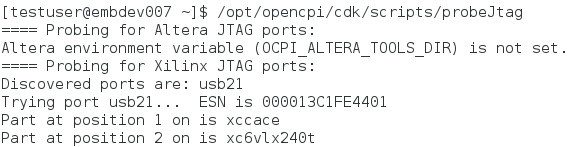
\includegraphics[scale=0.7]{./figures/probeJtag_success.jpg}}
%	\caption{Successful probeJtag}
%\end{figure}
%
%If you have an ANGRYVIPER bitstream ready to be deployed onto your target platform, you can follow these steps to test bitstream loading:
%\begin{enumerate}
%\item Set OCPI\_PROJECT\_PATH to the project containing the platform of interest. For example, to load bitstreams to the ML605, you will need to run:\\
%\code{export OCPI\_PROJECT\_PATH=\$OCPI\_PROJECT\_PATH:<path-to-baseproject>}
%
%\item Run ``\code{ocpihdl search}'' to determine the device of interest (i.e. PCI:XXXX:XX:XX.X for PCI platforms).
%\item Load a bitstream via USB-JTAG using ocpihdl:\newline
% \code{ocpihdl load -d PCI:XXXX:XX:XX.X <path-to-bitstream>}
%\end{enumerate}
%
\end{flushleft}
\pagebreak

\newpage

\section{Altera Toolset Installation and Configuration}
\subsection{Altera Quartus Prime 15.1 Installation in CentOS~7}
\begin{flushleft}
\begin{enumerate}
\item Download the Quartus Prime 15.1 installation files from Altera's download site: \url{https://www.altera.com/downloads/download-center.html}. A \verb+myAltera+ account will be required. This first page is the download-center home page. Select the \verb+Download+ button next to ``Quartus Prime sofware Standard edition" as shown in Figure \ref{fig:altera_download_center}.
\begin{figure}[ht]
	\centerline{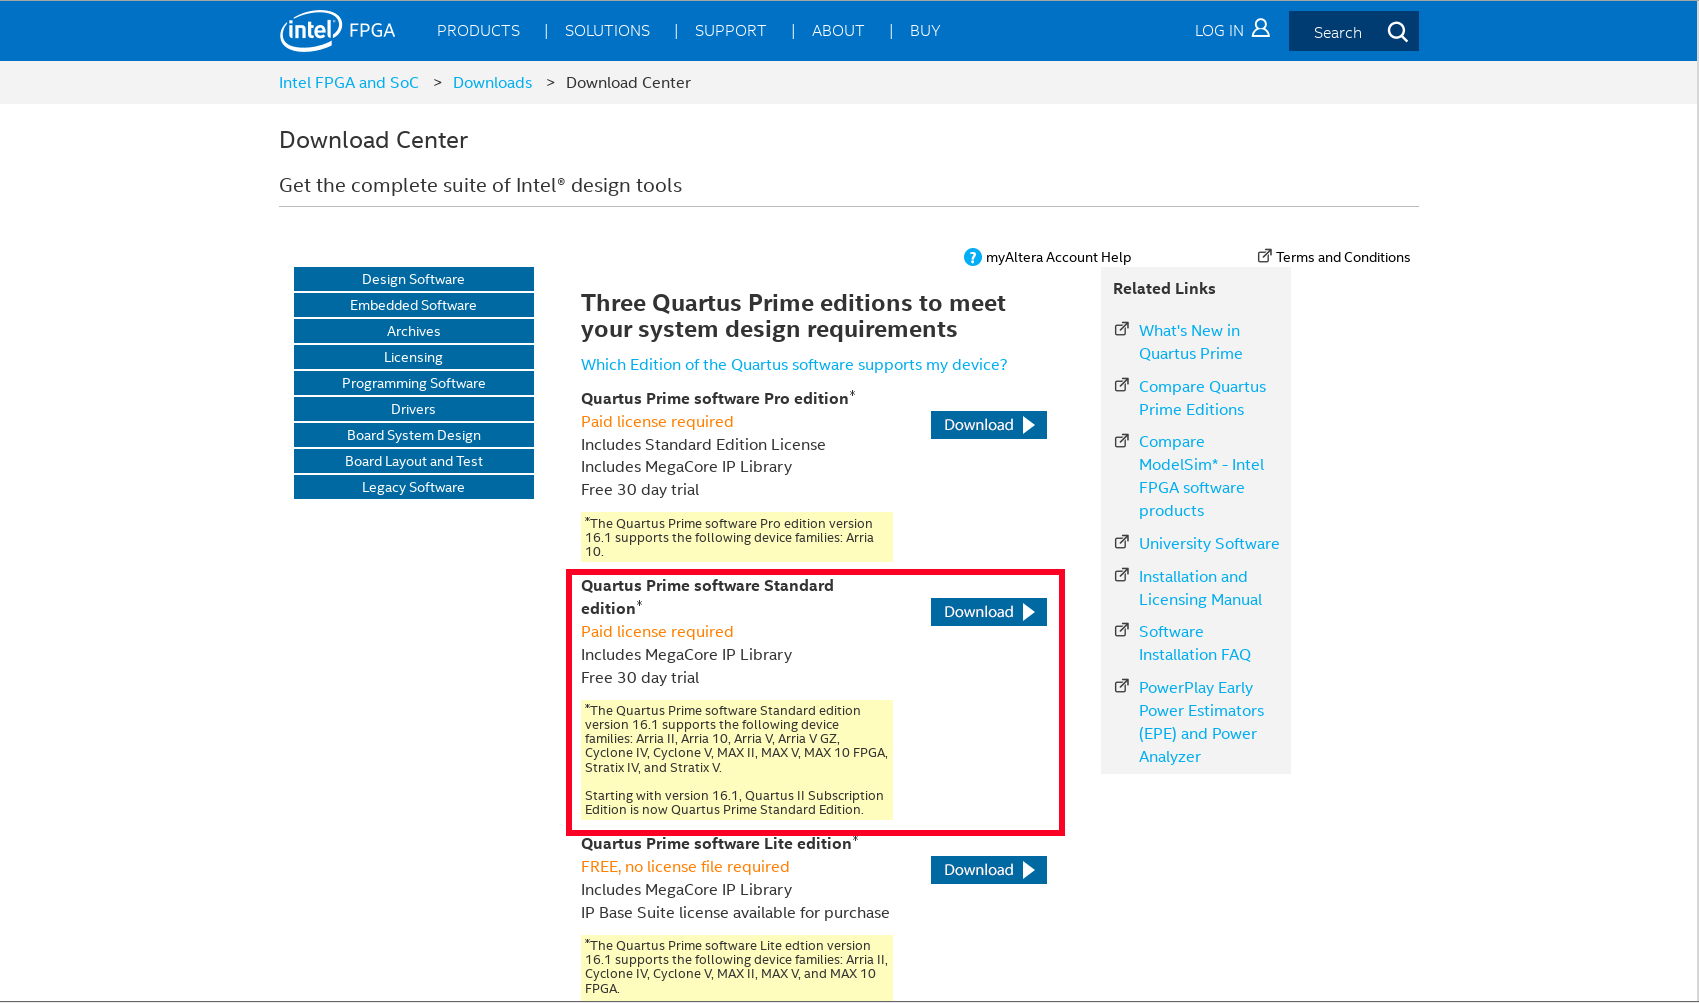
\includegraphics[scale=0.4]{figures/altera_download_center}}
	\caption{Altera Download Homepage}
	\label{fig:altera_download_center}
\end{figure}
\item From the ``Quartus Prime sofware Standard edition" page, select \verb+15.1+ from the drop-down box next to ``Select release" as shown in Figure \ref{fig:altera_download_15_1}.
\item Select the \verb+Complete Download+ version which downloads the file \verb+Quartus-15.1.0.185-linux-complete.tar+. Click the arrow pointing downward to begin the download as shown in Figure \ref{fig:altera_download_15_1}. Note that the tarball is $\sim$24GB. Ensure that the installation system has enough disk space and correct file write permissions.\pagebreak
\begin{figure}[ht]
	\centerline{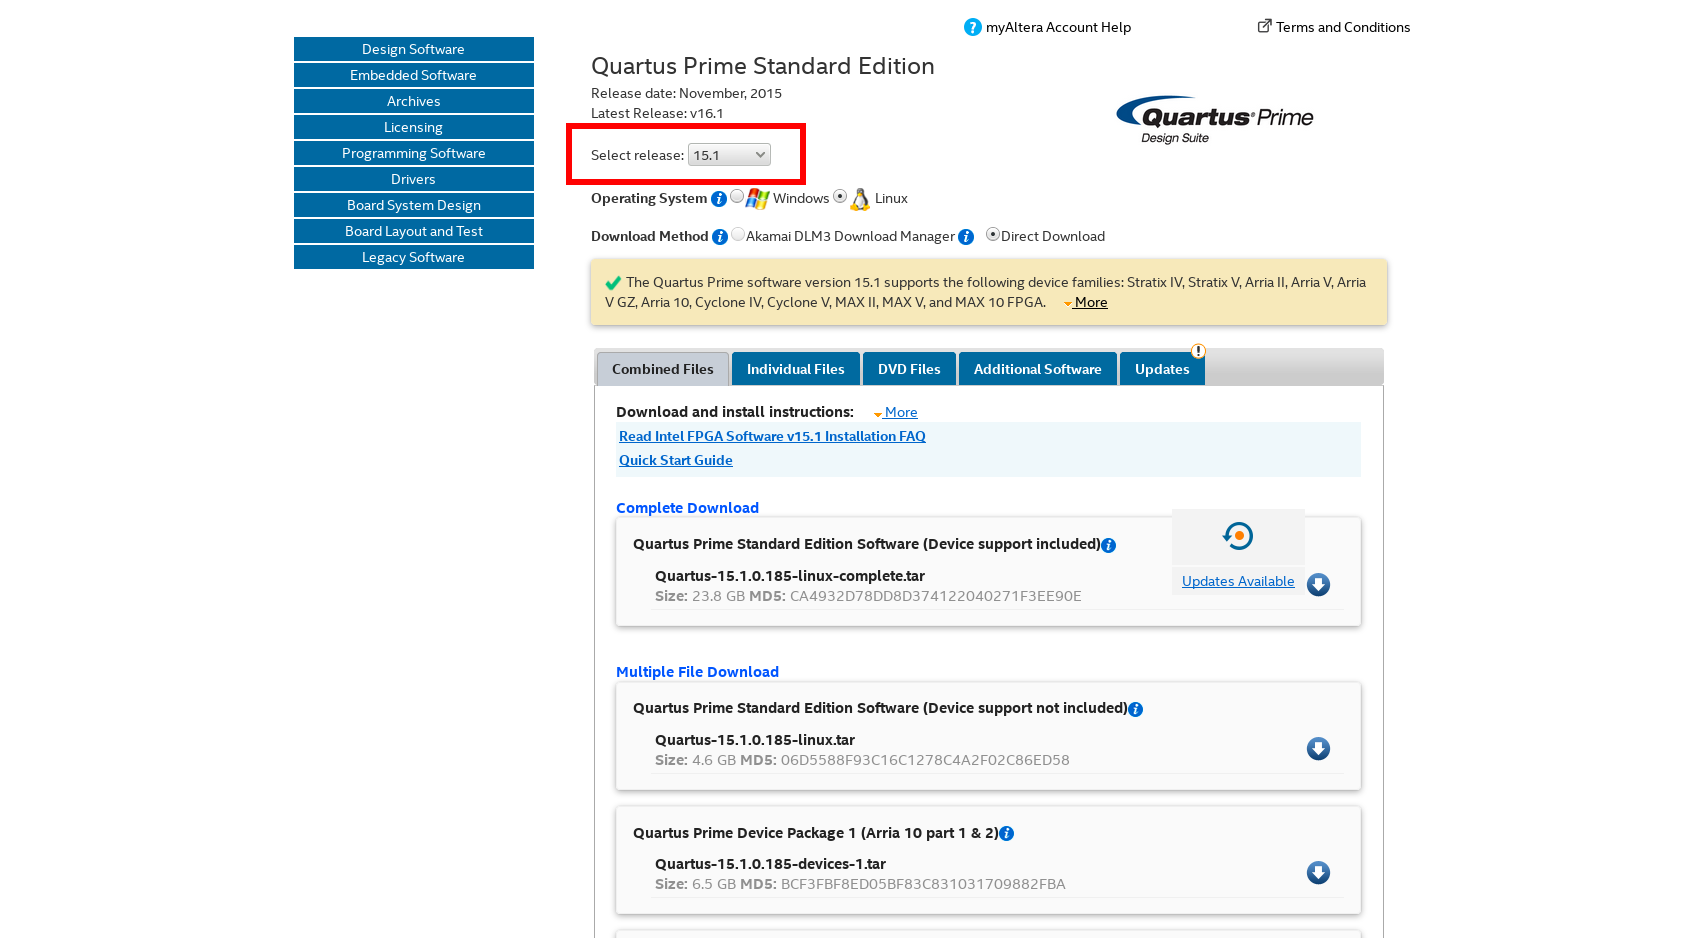
\includegraphics[scale=0.4]{figures/altera_download_15_1}}
	\caption{Altera Quartus Prime Standard Edition 15.1 Download}
	\label{fig:altera_download_15_1}
\end{figure}
\item Extract the tarball:\newline
\code{\% tar xvf Quartus-15.1.0.185-linux-complete.tar}\newline
Depending upon permissions of the current directory, execution of this command will likely require root privileges (i.e. \code{sudo}).
\item Run the installer:\newline
\code{\% ./setup.sh}\newline
Execution of this file will likely require root privileges (i.e. \code{sudo}).
\pagebreak
\item Run through the installation process. Refer to the images here when needed:
\begin{figure}[H]
	\centerline{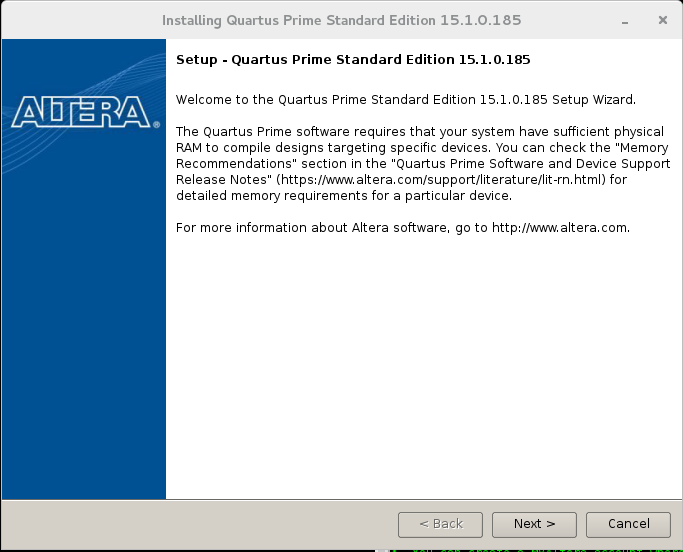
\includegraphics[scale=0.5]{figures/altera_install_1}}
	\caption{Altera Quartus Prime Setup Wizard}
\end{figure}

\begin{figure}[H]
	\centerline{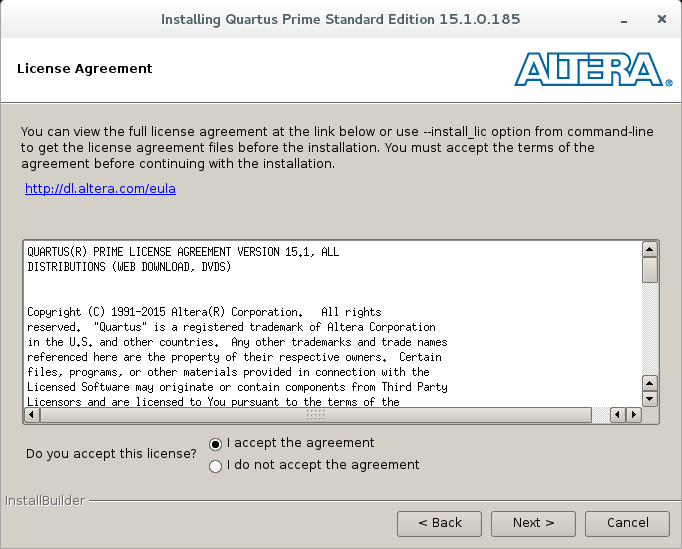
\includegraphics[scale=0.5]{figures/altera_install_2}}
	\caption{Altera Quartus Prime License Agreement}
\end{figure}
Take note of the installation directory chosen (e.g. \code{/opt/altera}) as well as the LabTools version (e.g. \code{15.1}) for later use.
\begin{figure}[H]
	\centerline{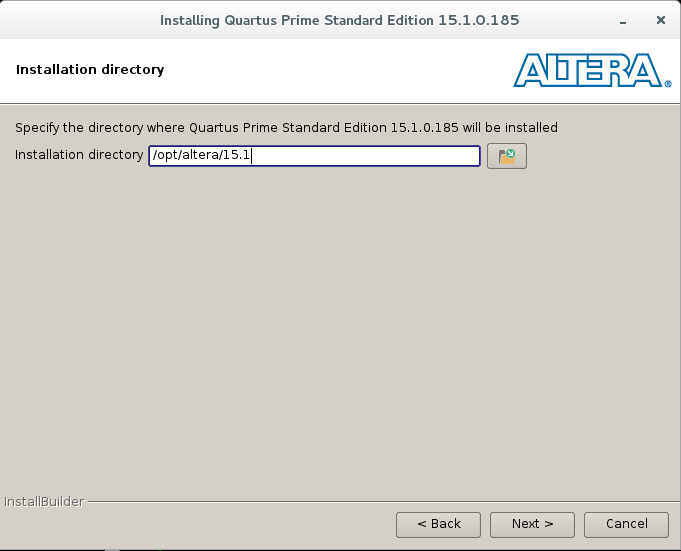
\includegraphics[scale=0.5]{figures/altera_install_3}}
	\caption{Altera Quartus Prime Installation Directory}
\end{figure}
\begin{figure}[H]
	\centerline{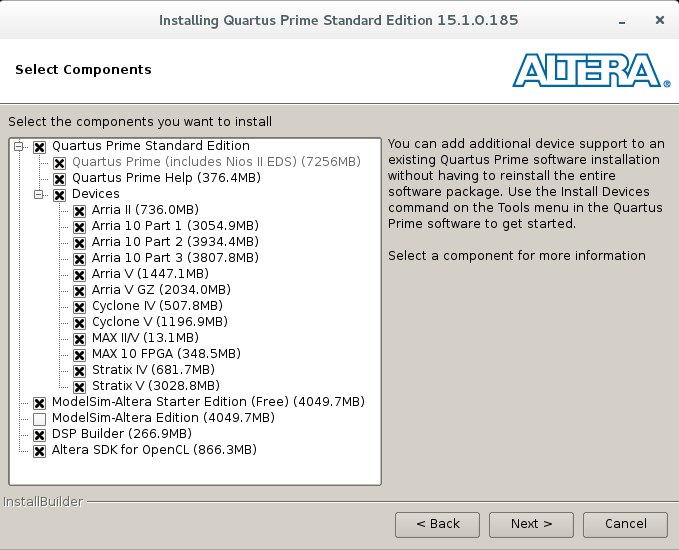
\includegraphics[scale=0.5]{figures/altera_install_4}}
	\caption{Altera Quartus Prime Select Components}
\end{figure}
\begin{figure}[H]
	\centerline{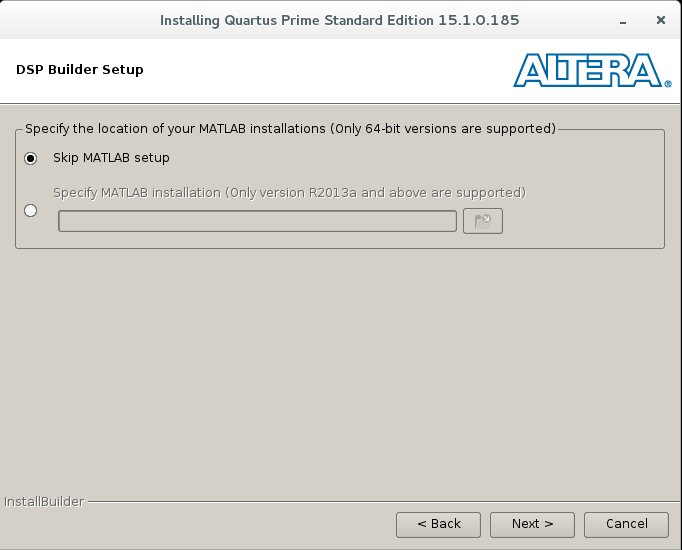
\includegraphics[scale=0.5]{figures/altera_install_5}}
	\caption{Altera Quartus Prime DSP Builder Setup}
\end{figure}
\begin{figure}[H]
	\centerline{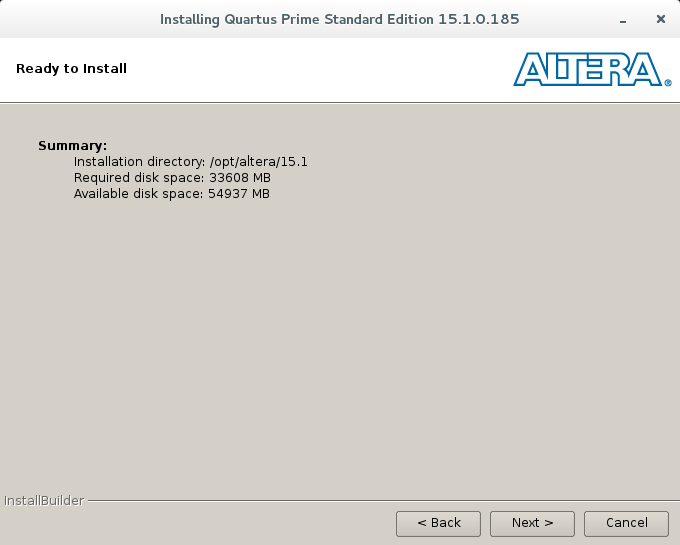
\includegraphics[scale=0.5]{figures/altera_install_6}}
	\caption{Altera Quartus Prime Installation Summary}
\end{figure}
\end{enumerate}


\subsubsection{ANGRYVIPER Considerations}
If ANGRYVIPER has been installed prior to the Quartus installation, it is required to set the following environment variables before running ANGRYVIPER commands. Note that \texttt{<altera-version>} should be replaced with the appropriate Altera version (e.g. \code{15.1}), and \texttt{<altera-install-dir>} should be replaced with the installation directory (i.e. \path{/opt/altera}). Note also that each of the following \code{export} statements are only necessary when the non-default installation location (i.e. anything other that \path{/opt/altera} or non-default version (i.e. anything other than \path{14.7}) of the tools were used.\newline
\code{\% export OCPI\_ALTERA\_DIR=<altera-install-dir>}\newline
\code{\% export OCPI\_ALTERA\_VERSION=<altera-version>}\newline
\code{\% export OCPI\_ALTERA\_LICENSE\_FILE=<path\_to\_license\_file>}

If ANGRYVIPER has been installed prior to the Quartus installation, and it is desired to make the environment variables set automatically upon login for all users, the variables should be added in \path{/opt/opencpi/cdk/env.d/altera.sh}. Logging out and logging back into the user account will apply said variables.

\subsection{Licensing Notes}
% AV-3316
If the user runs the Quartus software in its native GUI mode outside of ANGRYVIPER, a license file configuration \textit{might} be stored in the variable \path{LICENSE_FILE} within \path{~user/.altera.quartus/quartus2.ini}; this setting overrides the \code{OCPI\_ALTERA\_LICENSE\_FILE} noted above and may cause confusion.

\end{flushleft}

\end{document}
